
\section{Résultats sur l'implémentation}
\label{resultats}

	\subsection{Implémentation possible}
	
	Une des questions auxquelles nous devions répondre était la possibilité d'implémentation d'\textbf{UEDF}, qui 
	n'avait bénéficié jusque là d'aucune implémentation sur un RTOS.
	Le travail effectué a d'ores et déjà montré qu'il était possible de l'implémenter, ce qui est un premier résultat attendu.
	Il est néanmoins important de préciser que cette implémentation n'a pas atteint sa phase d'optimisation 
	et que la volonté dans ce travail a été avant toute chose d'avoir une implémentation fonctionnelle qui mettrait
	déjà en avant des caractéristiques intéressantes de cet ordonnanceur. 
	Le lecteur est d'autant plus invité à prendre les résultats non pas pour une affirmation générale 
	mais bien comme issue d'une première implémentation 
	\og{}exploratoire\fg{} qu'elle est observée en vis--à--vis d'une implémentation de \textbf{Global-EDF} déjà optimisée. 
	Nous donnerons des pistes d'amélioration dans le chapitre suivant. \newline
	
	\subsection{À la lisière entre théorie et pratique}
	
	Nous avons montré au chapitre \hyperref[contexte]{Contexte} [\ref*{contexte}] 
	que certains ensembles en théorie devraient être 
	ordonnançables par \textbf{UEDF }mais pas par\textbf{ Global-EDF}, cela en considérant les WCET comme 
	temps réels d'exécution. Dans la pratique --- comme on en a déjà parlé dans le chapitre \hyperref[methodo]{Méthodologie} [\ref*{methodo}] --- 
	les WCET ne doivent jamais être des temps d'exécution, et cette limite peut être plus ou moins éloignée 
	de la durée moyenne d'exécution d'une tâche. Nous avons également parlé du fait que l'ordonnanceur doit lui aussi
	être pris en considération pour paramétrer cet écart entre moyenne des temps d'exécution et WCET.\newline

	Nous avons souhaité tester deux ensembles afin d'illustrer notre propos ici. Ces ensembles sont
	 constitués respectivement de $6$ et $7$ tâches de périodes 
	non harmoniques, dont les hyper-périodes n'étaient pas excessivement grandes par rapport à la plus petite des périodes.
	\begin{itemize}
		\item Hyper-période = $6$ fois la plus petite période pour le premier ensemble
		\item Hyper-période = $8$ fois la plus petite période pour le second
	\end{itemize}
	Ces ensembles, en théorie, ne devraient pas être ordonnancés par \textbf{Global-EDF}, si les WCET étaient peu éloignés du temps 
	moyen d'exécution.\newline
	
	
	\subsubsection{Répartition de charge de travail}
	Une première analyse de la répartition de charge de travail sur les $4$ cœurs, en fonction de l'ordonnanceur, 
	ne montre pas de grande différence, comme on peut en juger sur \hyperref[3tasksmigrations]{la figure 6.2}.
	
	\begin{figure}[H]
		\label{3tasksmigrations}
		\caption{Comparaison charges de travail \textbf{UEDF}, \textbf{Global-EDF}}
		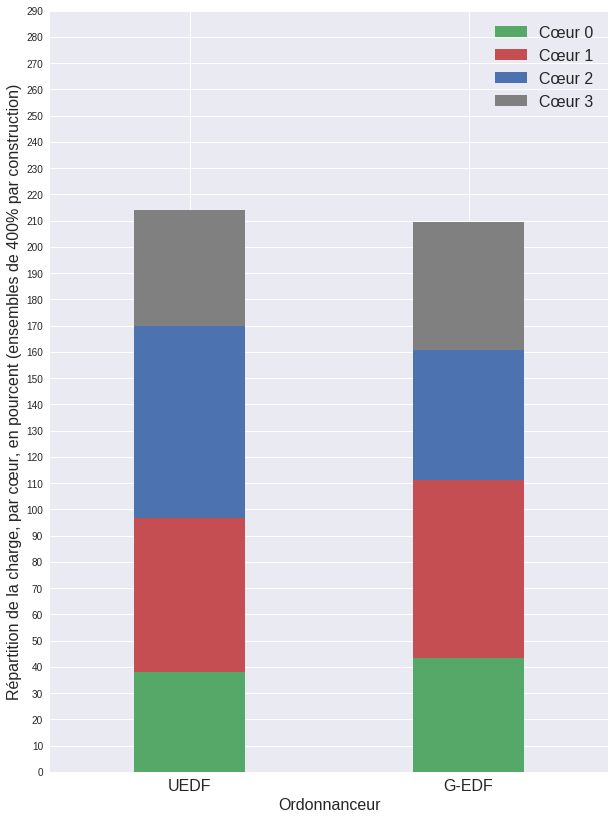
\includegraphics[scale=0.6]{img/wcet/repartitiondecharges_migrations.png}
	\end{figure}
	
	La charge totale du système est proche de $200\%$. La différence qui s'observe 
	entre les deux totaux s'explique par les légères variations d'une exécution à une autre, or notre échantillon est 
	petit pour cette expérience puisque nous n'avons que deux ensembles par ordonnanceur, le but n'étant pas de 
	généraliser mais bien de montrer un type de comportement qui a de l'influence.\newline
	
	
	\subsubsection{Nombre de migrations}
	
	En l'absence d'optimisations qui empêchent ce comportement, par défaut,\textbf{UEDF} va provoquer un nombre 
	important de migrations, tandis que dans le même temps, \textbf{Global-EDF} n'en produit aucune.
	Sur les deux ensembles, nous avons souhaité rendre compte du nombre de migrations en calculant 
	ce nombre d'événements sur l'hyper-période, que nous nommons \og{}densité de migration\fg{}, qui est 
	la somme des migrations durant l'hyper-période divisée par le nombre de tâches. 
	Nous trouvons, pour \textbf{UEDF} : 
	\begin{enumerate}
		\item 10 migrations par hyper-période pour le premier ensemble de 6 tâches, soit une densité de $1,66$
		\item 6 pour le second, de 7 tâches soit une densité de $0,85$
		\item aucune pour \textbf{Global-EDF} dans aucun des deux systèmes
	\end{enumerate}

	Les migrations vont provoquer du surcoût. Ce surcoût doit être intégré dans le paramétrage du WCET. 
	Ceci explique pourquoi en l'état actuel de l'implémentation, et avec ce type d'ensembles de tâches 
	de périodes non harmoniques, \textbf{UEDF} ne montre pas sa 
	supériorité par rapport à \textbf{Global-EDF}, on peut même dire l'inverse, car 
	la répartition de charge est légèrement meilleure pour \textbf{Global-EDF}, qui déploie 
	beaucoup moins d'efforts et de calculs qu'\textbf{UEDF} pendant le même temps.\newline
	
	
	\section{Temps passé dans l'algorithme}
	
	Nous avons voulu vérifier l'évolution du temps passé dans la fonction $ComputeSchedule$, qui nous semblait critique 
	au début de ce travail. Nous présentons ici un schéma qui montre 
	l'évolution du temps passé pour $1$ unité d'exécution dans cette fonction. C'est donc la 
	proportion de temps passée dans cette fonction par rapport au nombre de tâches. \newline
	Cette expérience n'a été réalisée qu'avec des ensembles de $100$\% d'utilisation.

	\begin{figure}[H]
	\label{timeevolution}
		\caption{Évolution du temps passé dans ComputeSchedule, \textbf{UEDF}}
		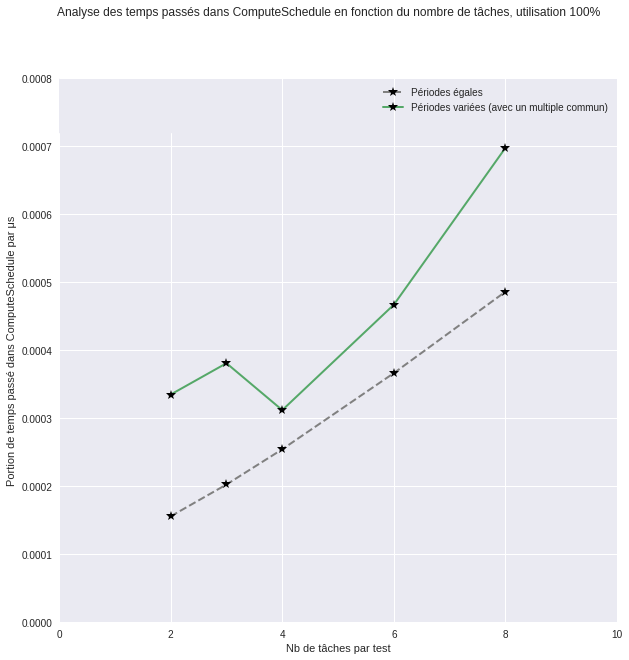
\includegraphics[scale=0.5]{img/wcet/elapsedInCompueSchedule}
	\end{figure}		

	On voit bien que ce temps évolue, néanmoins, il reste à des valeurs qui nous semblent totalement acceptables.
	Nous pensons donc qu'il est plus important de viser de diminuer les préemptions et autres migrations que 
	d'optimiser --- du moins en premier lieu --- cette partie du code.
	
	
\section{Ensembles variés dont la somme d'utilisation est de 400 \%}

	\subsection{UEDF}
	Dans les expériences suivantes, nous avons constitué un nombre variable d'ensembles de $6$, $8$,; $10$ et $12$ tâches, 
	et avons procédé à l'analyse de la répartition de charge des processeurs.\newline
	
	Les expériences précédentes nous ont mené à produire des ensembles constitués de 
	périodes harmoniques, ou \og{}presque\fg{}. Ainsi, pour éviter d'avoir des 
	périodes extrêmement longues, certaines périodes ont des multiples communs 
	avec les autres périodes mais ne sont pas directement multiples. Leur nombre est limité, aussi, nous pouvons 
	caractériser ces ensembles de \og{}simples\fg{}.\newline

	\begin{figure}[H]
		\label{loadevolution}
		\caption{Comparaison charges de travail \textbf{UEDF}}
		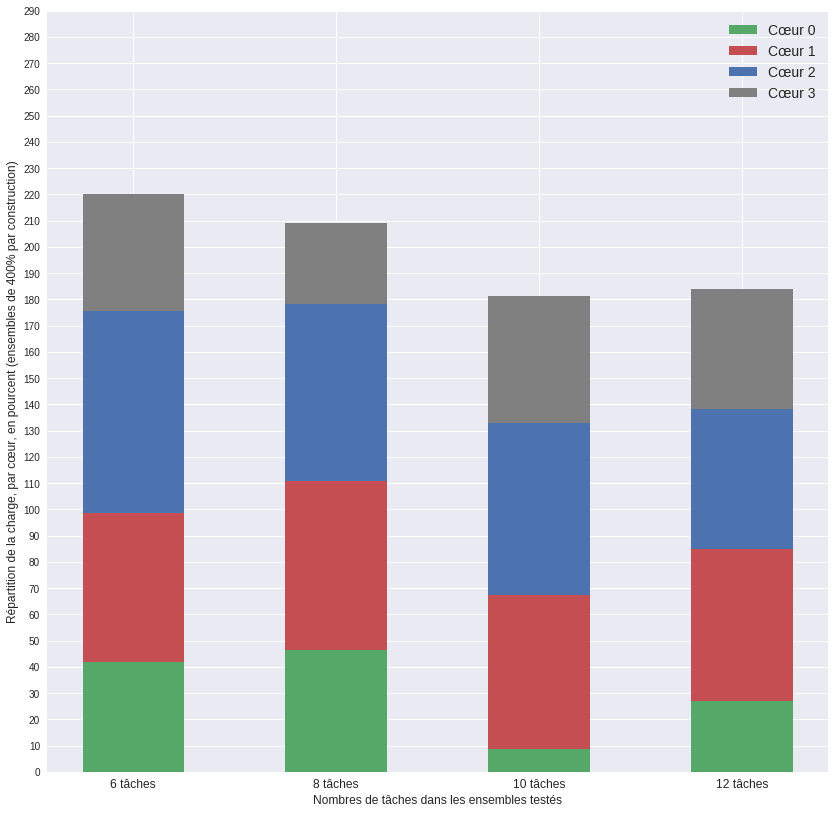
\includegraphics[scale=0.5]{img/wcet/repartitiondecharges_uedf}
	\end{figure}		
	
	La charge moyenne, dans ce cas, dépasse de peu les $200\%$, ce qui semble plutôt convenable. \newline
	
	Un phénomène apparaît, cependant, qui est une charge moins importante pour le premier cœur que pour les autres, et également 
	moins importante pour le dernier cœur. Cela s'explique facilement : 
	\begin{itemize}
		\item Nous avons volontairement été pessimiste avec les tâches de périodes les plus petites qui s'exécutent sur le 
		premier cœur car c'est le \textit{Master}, aussi une grande partie des surcoûts pèsent sur sa charge totale.
		\item D'après le fonctionnement d'\textbf{UEDF}, le dernier cœur est chargé d'exécuter les travaux d'échéances les plus 
		éloignées, aussi, comme les écarts entre les temps moyens et les WCET sont de près du simple au double, 
		le travail sera souvent terminé voire très avancé dans son exécution lorsqu'il sera déployé sur le dernier cœur.
	\end{itemize}

	\subsection{Global-EDF}
	
	Nous avons rejoué les mêmes ensembles en utilisant cette fois \textbf{Global-EDF}. Nous pouvons constater que 
	la charge totale est répartie différemment, puisqu'au contraire d'\textbf{UEDF}, nous ne voyons pas spécialement d'écart 
	entre les cœurs : la répartition est équitable entre tous les cœurs. 
	
	\begin{figure}[H]
	\label{loadevolutionGEDF}
	\caption{Comparaison charges de travail \textbf{Global-EDF}}
	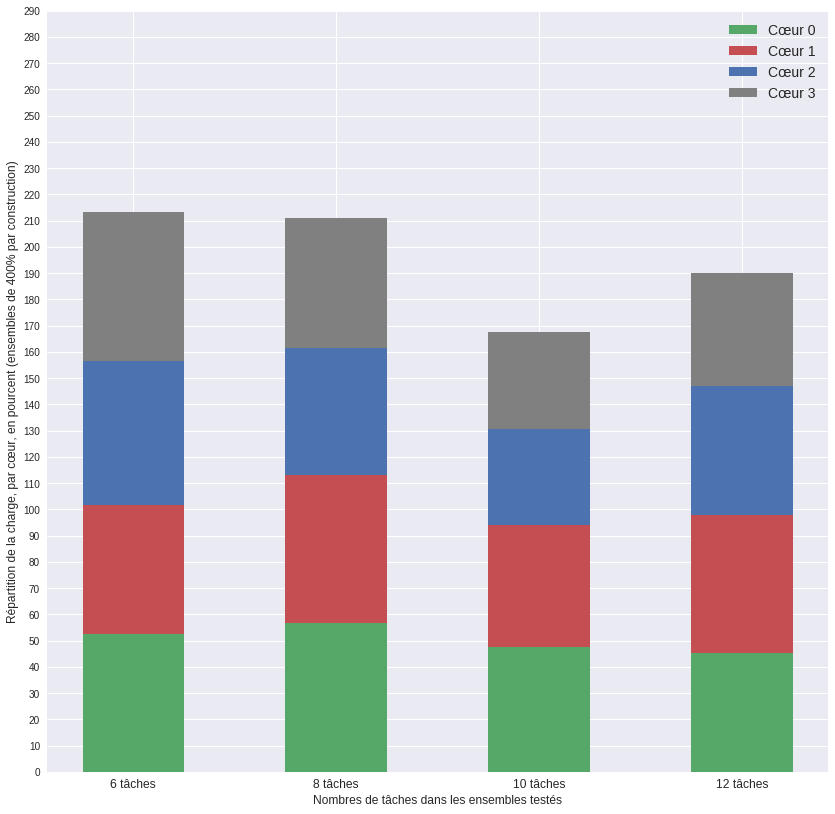
\includegraphics[scale=0.5]{img/wcet/repartitiondecharges_gedf}
	\end{figure}		

	Pour cette expérience encore, la supériorité d'\textbf{UEDF} n'a pas été démontrée.
	En revanche, comme nous en parlerons dans la partie \hyperref[contexte]{Perspectives} [\ref*{perspectives}], en procédant à quelques changements dans l'implémentation, 
	nous pensons que ces résultats peuvent grandement s'améliorer, et en fin de compte, ces premiers indices peuvent être 
	considérés comme prometteurs pour la suite.

		
		

	